% article example for classicthesis.sty
\documentclass[10pt,a4paper]{article} % KOMA-Script article scrartcl
\usepackage{import}
\usepackage{xifthen}
\usepackage{pdfpages}
\usepackage{transparent}
\newcommand{\incfig}[1]{%
    \def\svgwidth{\columnwidth}
    \import{./figures/}{#1.pdf_tex}
}
\usepackage{lipsum}     %lorem ipsum text
\usepackage{titlesec}   %Section settings
\usepackage{titling}    %Title settings
\usepackage[margin=10em]{geometry}  %Adjusting margins
\usepackage{setspace}
\usepackage{listings}
\usepackage{amsmath}    %Display equations options
\usepackage{amssymb}    %More symbols
\usepackage{xcolor}     %Color settings
\usepackage{pagecolor}
\usepackage{mdframed}
\usepackage[spanish]{babel}
\usepackage[utf8]{inputenc}
\usepackage{longtable}
\usepackage{multicol}
\usepackage{graphicx}
\graphicspath{ {./Images/} }
\setlength{\columnsep}{1cm}

% ====| color de la pagina y del fondo |==== %
\pagecolor{white}
\color{black}



\begin{document}
    %========================{TITLE}====================%
    \title{{  Preparcial 2 Teoría de grafos  }}
    \author{{Rodrigo Castillo}}
    \date{\today}

    \maketitle


     % ====| Loguito |==== %
    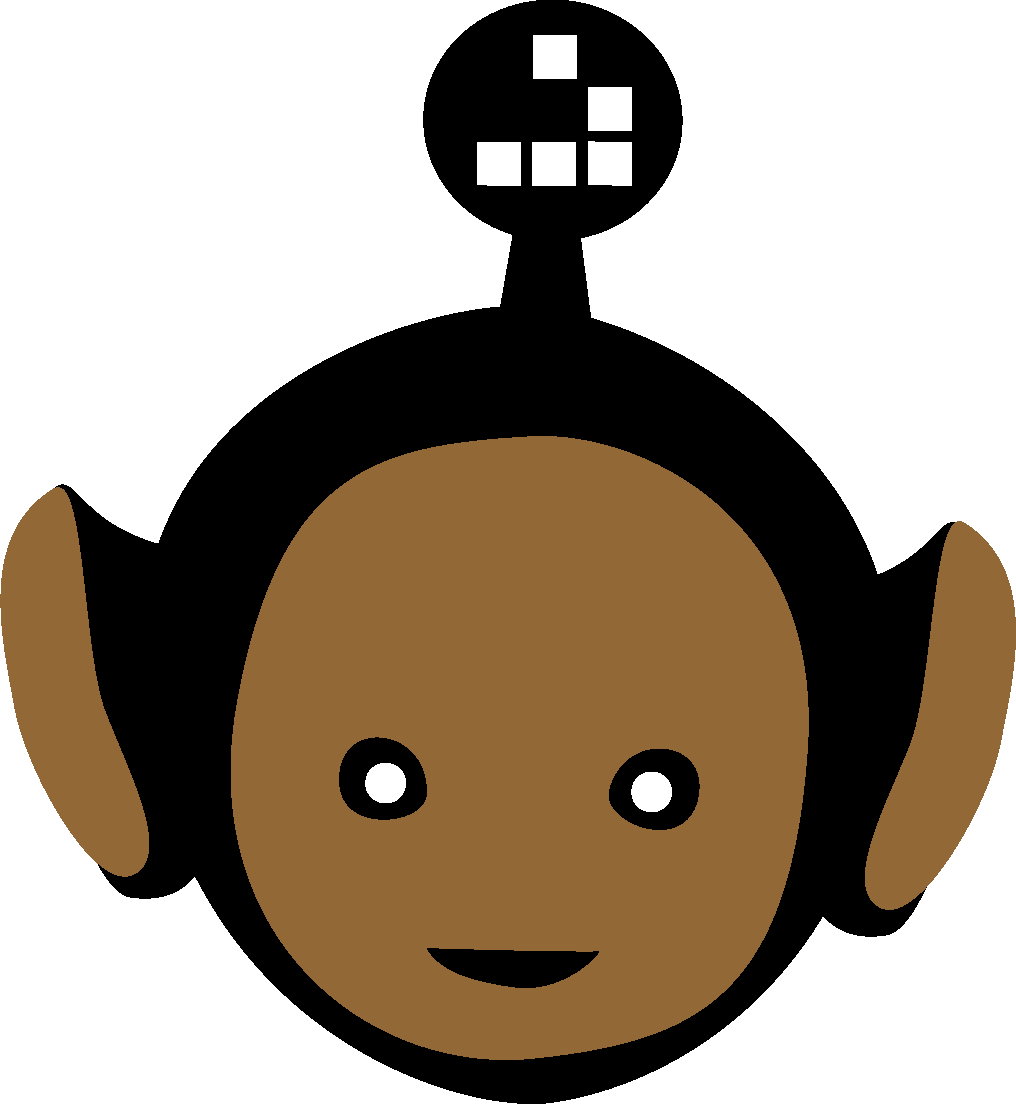
\includegraphics[width=0.1\linewidth]{negro_cara.png}
    %=======================NOTES GOES HERE===================%
    \section{sean $x$ y $y$ vertices adyacentes en un grafo conexo , $G$ , para
    todo $z$ en $V(G)$  demuestre que :}
    \begin{equation}
        |d_G (x,z) - d_G (y,z) <=1 |
    \end{equation}
    \textbf{Demostración:}
    % ====|ACA EMPIEZA EL PUNTO 1|====



    % ====|ACA TERMINA EL PUNTO 1|==== %

    \section{Considere el grafo $G_1$ }
        \begin{center}
        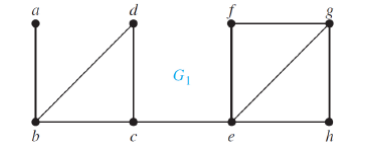
\includegraphics[width=0.4\linewidth]{grafop2.png}
        \end{center}
        \begin{center}
        \begin{enumerate}
            \item {escriba la excentricidad de cada vértice y calcule $rad(G_1)$ y $diam(G_1)$}
            \item {encuentre el centro de $G_1$ y calcule el índice de $Wiener$
                y la distancia promedio}
        \end{enumerate}
        \end{center}
        % ====|ACA EMPIEZA EL PUNTO 2|====



        % ====|ACA TERMINA EL PUNTO 2|==== %

    \section{Calcule el centro y el radio del biclicke $K_{m,n}$}
        % ====|ACA EMPIEZA EL PUNTO 3|====



        % ====|ACA TERMINA EL PUNTO 3|==== %

    \section{Encuentre el código de Prufer del siguiente arbol:}
        \begin{center}
            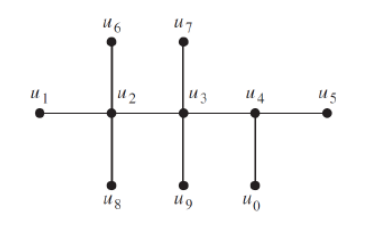
\includegraphics[width=0.4\linewidth]{arbolp4}
        \end{center}
        % ====|ACA EMPIEZA EL PUNTO 4|====



        % ====|ACA TERMINA EL PUNTO 4|==== %

    \section{Construya el arbol $T$ a partir del código de Prufer $322114211$}
        % ====|ACA EMPIEZA EL PUNTO 5|====



        % ====|ACA TERMINA EL PUNTO 5|==== %


    \section{Determine cuáles árboles tiene código de prufer que $(a)$
    contienen un valor , $(b)$ contienen exactamente 2 valores , $(c)$ tienen
    distintos valores en todas las posiciones}
        % ====|ACA EMPIEZA EL PUNTO 6|====



        % ====|ACA TERMINA EL PUNTO 6|==== %

    \section{Determine el número de árboles de expansión del siguiente grafo...}
       \begin{center}
            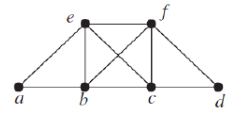
\includegraphics[width=0.5\linewidth]{grafop7.png}
       \end{center}

       % ====|ACA EMPIEZA EL PUNTO 7|====



       % ====|ACA TERMINA EL PUNTO 7|==== %

   \section{Calcule $ r(K_{m,n})$}
        % ====|ACA EMPIEZA EL PUNTO 8|====



        % ====|ACA TERMINA EL PUNTO 8|==== %

   \section{Utilice la búsqueda a profundidad y la búsqueda a lo ancho para
   encontrar árboles de expansión del siguiente grafo. Tome como vértice
   inicial $(a)$ y a $(b)$ como vértice  j, $(c)$ como vértice s}
       \begin{center}
       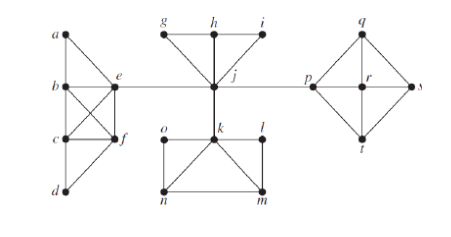
\includegraphics[width=0.5\linewidth]{grafop9.png}
       \end{center}
        % ====|ACA EMPIEZA EL PUNTO 9|====



        % ====|ACA TERMINA EL PUNTO 9|==== %

   \section{considere el grafo ponderado:}
        \begin{center}
            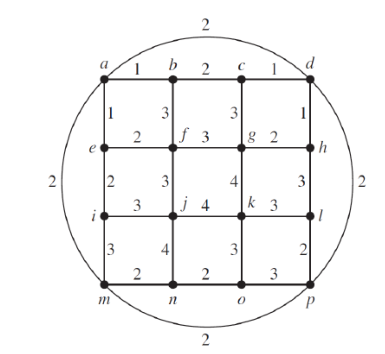
\includegraphics[width=0.4\linewidth]{grafop10}
        \end{center}
        \begin{enumerate}
            \item {utilice el algoritmo de Prim para encontrar el árbol de
                expansión mínimo}
            \item {Utilice el algoritmo de Kruskal para encontrar el árbol de expansión máximo}
            \item {Utilice el algoritmo de Dijkstra para encontrar la ruta
                mínima entre los vértices $a$ y $p$}
        \end{enumerate}
        % ====|ACA EMPIEZA EL PUNTO 10|====



        % ====|ACA TERMINA EL PUNTO 10|==== %

        \section{Hay cinco ciudades en una red , el tiempo para viajar
        directamente de $i$ a $j$ es la entrada $a_{ij}$ , de la siguiente
        matrix. La matriz no es simétrica. (Use un grafo dirigido) y $a_{ij}$ =
        $\infty$ significa que no existe una ruta directa entre $i$ y $j$ Use el
        algoritmo de $Floyd-Warshall$ para encontrar la ruta mas rápida entre $i$ y $j$
        para cada par $i,j$  }
            \begin{center}
                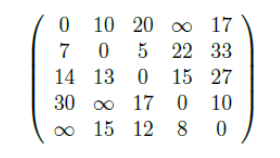
\includegraphics[width=0.4\linewidth]{matrixp11.png}
            \end{center}
            % ====|ACA EMPIEZA EL PUNTO 11|====



            % ====|ACA TERMINA EL PUNTO 11|==== %

        \section{Considere la siguiente tabla de frecuencias}
            \begin{center}
                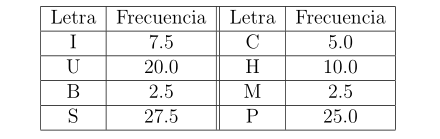
\includegraphics[width=0.4\linewidth]{tabfrec12.png}
            \end{center}

            \begin{enumerate}
                \item {Construya un código de Huffman y codifique la cadena $PMUBSCH$}
                \item {calcule la longitud esperada y la entropía}
                \item {Decodifique la cadena esa re larga que dan ahí}
            \end{enumerate}

            % ====|ACA EMPIEZA EL PUNTO 12|====



            % ====|ACA TERMINA EL PUNTO 12|==== %

        \section{Escriba los recorridos pre orden , post orden y in orden del siguiente arbol:}
            \begin{center}
                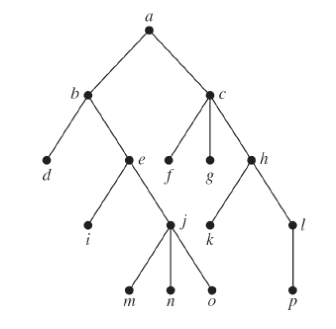
\includegraphics[width=0.4\linewidth]{arbolp13.png}
            \end{center}

            % ====|ACA EMPIEZA EL PUNTO 13|====



            % ====|ACA TERMINA EL PUNTO 13|==== %

        \section{escriba las siguientes formulas en notación infija:}
            \begin{center}
                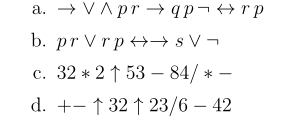
\includegraphics[width=0.5\linewidth]{form14.png}
            \end{center}
            % ====|ACA EMPIEZA EL PUNTO 14|====



            % ====|ACA TERMINA EL PUNTO 14|==== %

        \section{Considere el siguiente grafo $G$}
            \begin{center}
                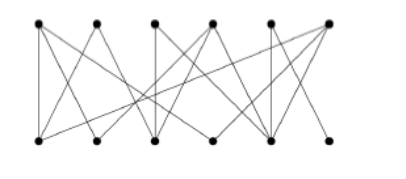
\includegraphics[width=0.4\linewidth]{ultimografo.png}
            \end{center}

            \begin{enumerate}
                \item {verifique si cumple la condición de Hall}
                \item {ecuentre el emparejamiento máximo (justifiquelo
                    mostrando un cubrimiento por vértices minimo)}
                \item {encuentre un emparejamiento maximal que no sea máximo}
                \item {encuentre un conjunto independiente máximo }
                \item {encuentre un cubrimiento por aristas mínimo}
            \end{enumerate}

            % ====|ACA EMPIEZA EL PUNTO 15|====



            % ====|ACA TERMINA EL PUNTO 15|==== %



            % ====| ACA SE ACABA LA FUCKING TAREA!!!!! |==== %
    %=======================NOTES ENDS HERE===================%

    % bib stuff
    \nocite{*}
    \addtocontents{toc}{{}}
    \addcontentsline{toc}{section}{\refname}
    \bibliographystyle{plain}
    \bibliography{../Bibliography}
\end{document}
